\chapter{Einleitung}

In der Industrie gewinnt Vernetzbarkeit immer mehr an Bedeutung. So lässt sich zum Beispiel durch das Vernetzen von externen Geräten mit den Produktionsmaschinen die Arbeitseffizienz erhöhen. Um diese Kommunikation zu vereinfachen und zu verbessern, wurde das Process Field Network (\gls{profinet}), eine Protokollfamilie, entwickelt.\\
\gls{profinet} setzt auf Ethernet für echtzeitfähige Anwendungen auf, und auf \gls{tcp}/\gls{ip} für langsamere \gls{io} Anwendungen. Durch die immer mehr vernetzten und oft dem Internet zugänglichen Produktionsstätten ist Sicherheit mittlerweile von höchster Bedeutung. \par
Dieses Projekt setzt an dieser Stelle an und soll dem \gls{ids} \gls{snort} ermöglichen, die \gls{profinet} Protokolle zu verstehen und zu verarbeiten. Zu diesem Zweck soll ein \gls{praeprozessor} für \gls{profinet} entwickelt werden. Um dem Benutzer eine Übersicht über die stattfindenden Kommunikationsprozesse zu verschaffen, soll zusätzlich eine \gls{gui} entwickelt werden. Diese soll mithilfe verschiedener Graphalgorithmen eine geordnete Darstellung ermöglichen.\par
Die Abbildung~\ref{fig:diagram} zeigt im unteren Teil den \gls{profinet} \gls{praeprozessor}, welcher \gls{snort} die Dekodierung von \gls{profinet} Paketen ermöglicht. Die dekodierten \glspl{paket} werden per \gls{ipc} zum \gls{programname} Prozess gesendet. Wobei der \gls{programname} Prozess als \textit{CLIENT} die Dienste des \textit{SERVER}s \gls{snort} in Anspruch nimmt (Client-Server-Modell).\\
\Gls{programname} selbst ist nach dem \gls{mvc} Prinzip strukturiert.\\
Das \textit{MODEL} holt die Pakete von der \gls{ipc} Schnittstelle. Sobald neue Daten zur Verfügung stehen werden diese in die vorhandene Datenstruktur eingeordnet und der \textit{VIEW} wird mitgeteilt, dass \textit{neue Daten} zur Verfügung stehen. \textit{VIEW} holt daraufhin die neuen Daten und präsentiert sie entsprechend auf der \gls{gui}.\\
\textit{Benutzereingaben} im \textit{VIEW} werden dem \textit{CONTROLLER} gemeldet. Dieser erzeugt \textit{Feedback} im \textit{VIEW} welches vom Benutzer wahrgenommen werden kann. Der \textit{CONTROLLER} hat außerdem die Möglichkeit durch Benutzerbefehle oder andere Geschäftslogiken induzierte Manipulationen am \textit{MODEL} vorzunehmen.

\begin{figure}[h]
  \centering
  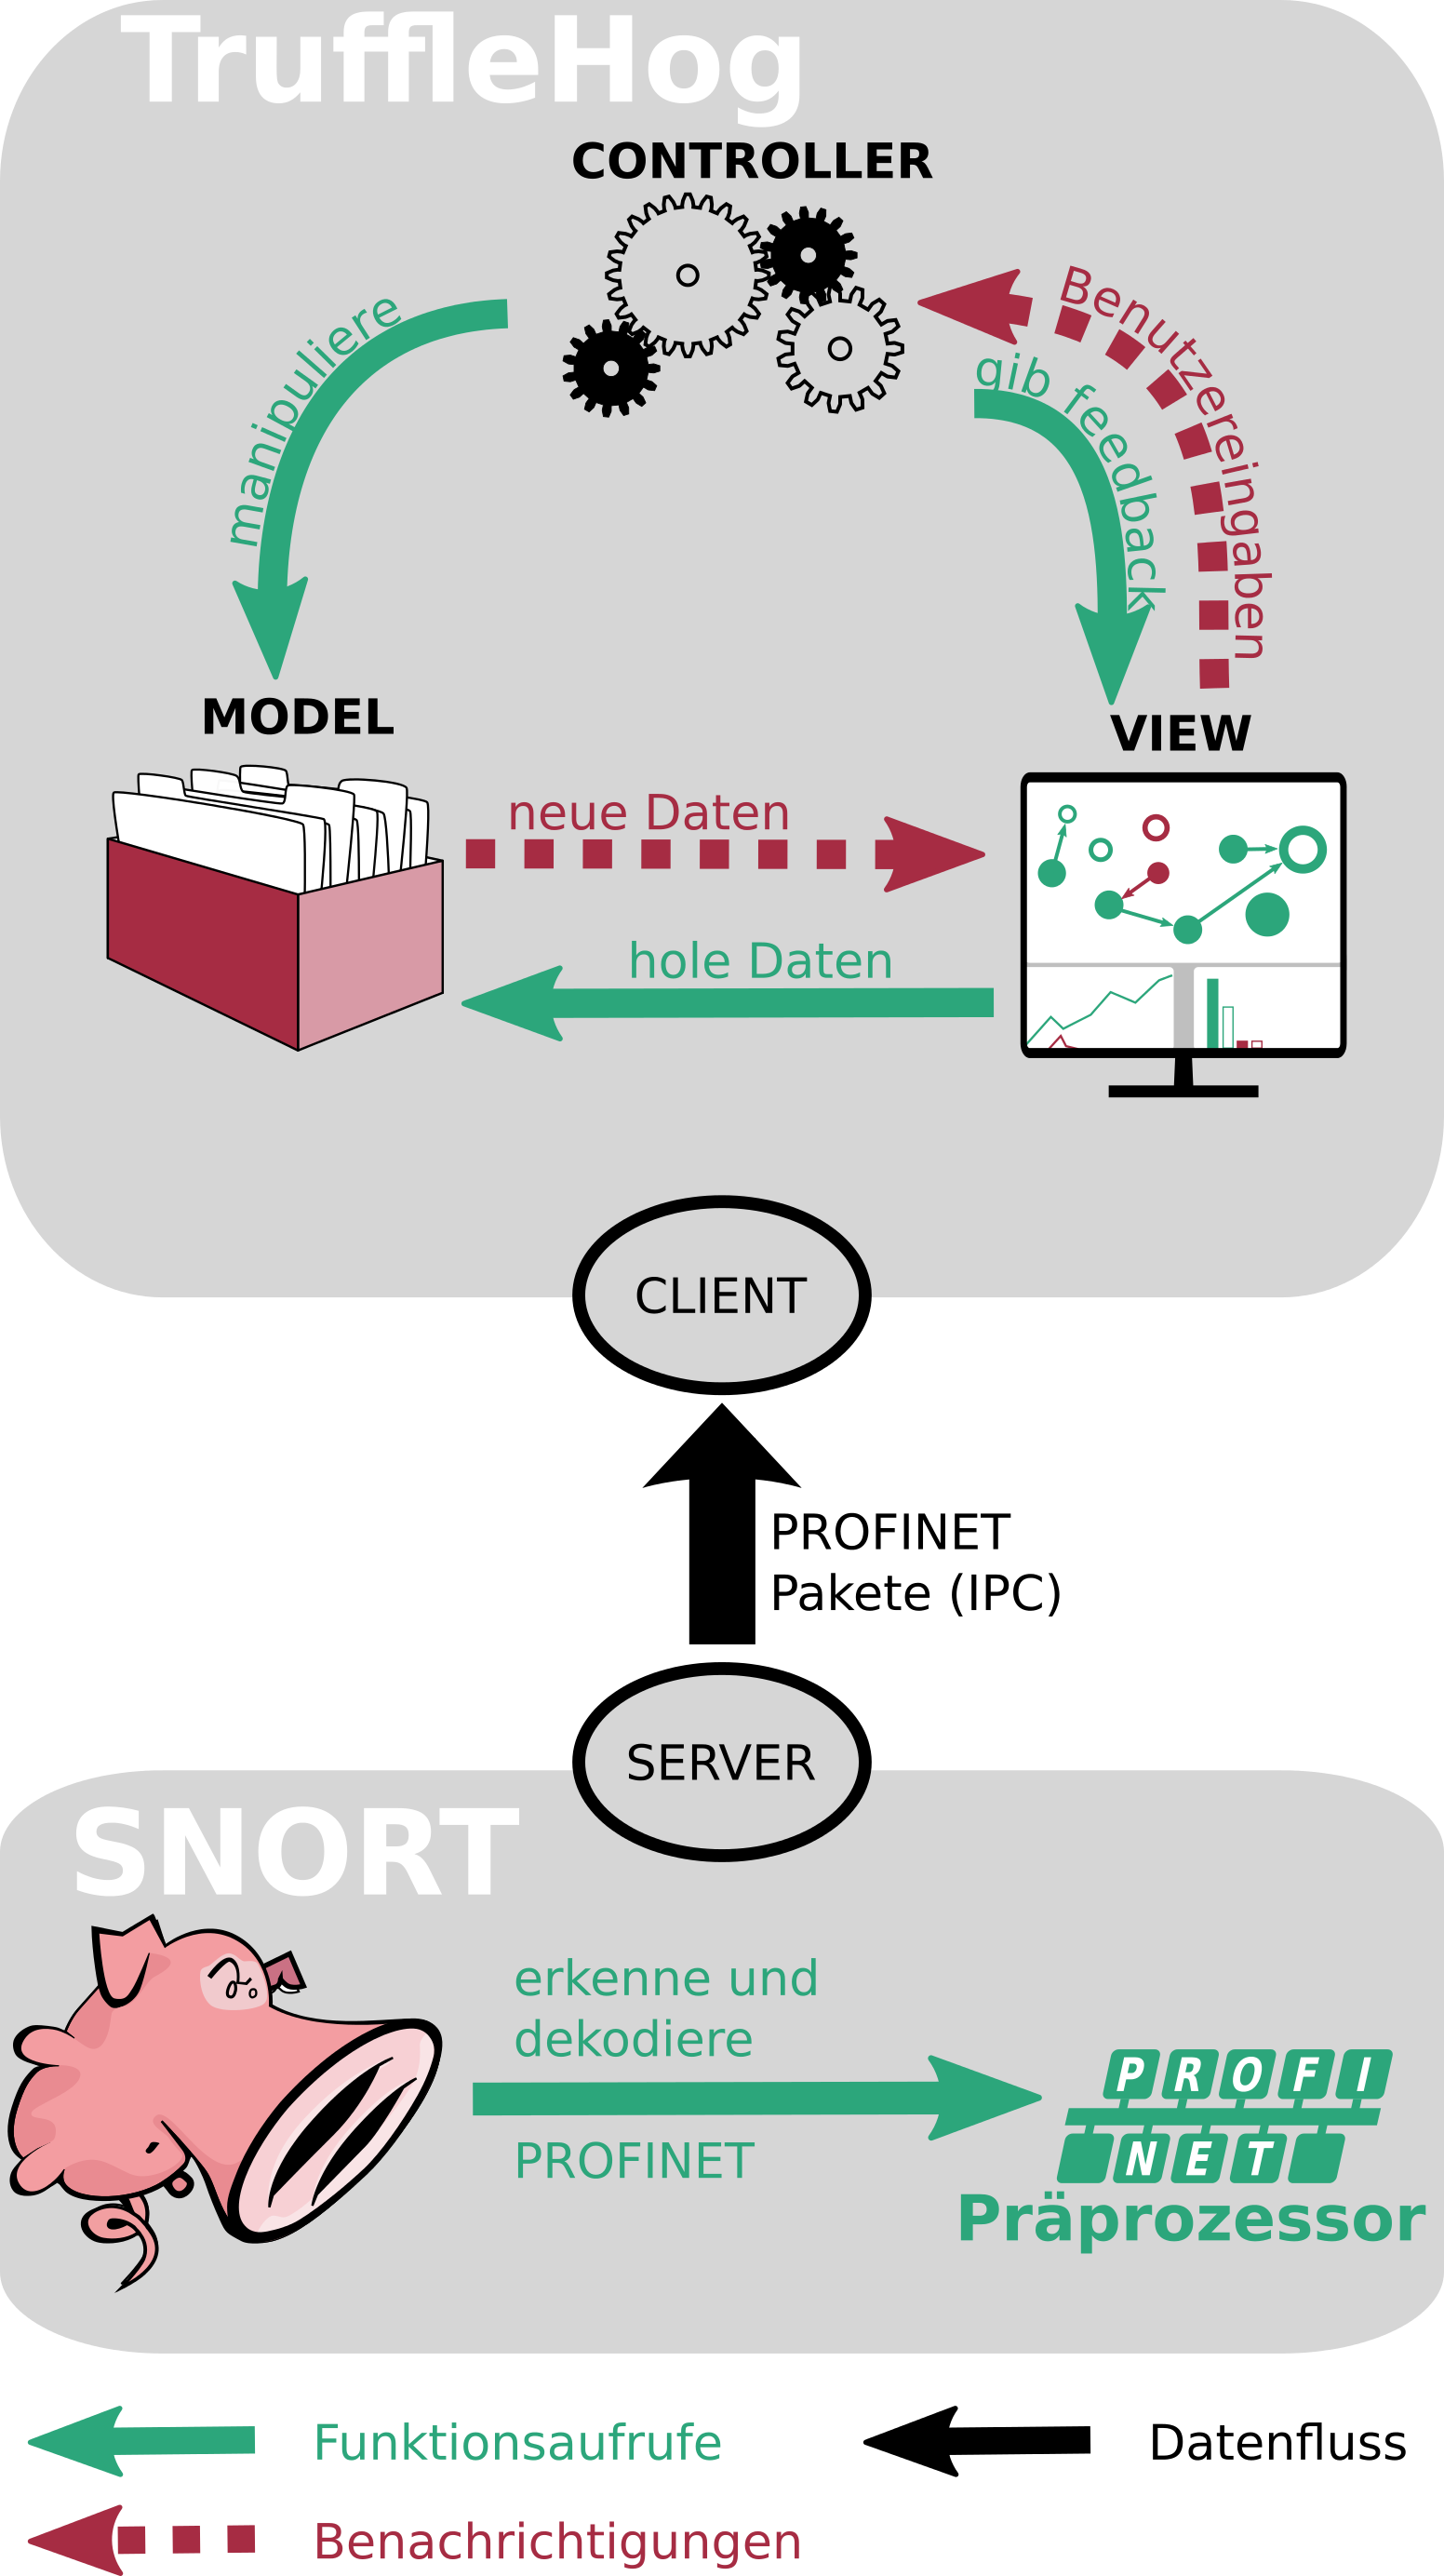
\includegraphics[width=300pt]{../diagrams/intro_diagram/intro_diagram.png}
  \caption[Strukturübersicht des Projekts]{Strukturübersicht des Projekts}\label{fig:diagram}
\end{figure}